\documentclass[a0,portrait]{a0poster}
%%%Load packages
\usepackage{tipa}
\usepackage{amsmath}
\usepackage{enumerate}
\usepackage{graphicx}
\usepackage{float}
\usepackage[scriptsize]{subfigure}
\usepackage{caption}
\usepackage{multirow}
\usepackage{color}
\usepackage{natbib}
\usepackage{ragged2e}
\usepackage{multicol} 			%3-column layout
\usepackage[left=3cm,right=3cm,bottom=0cm,top=0cm]{geometry}			%Reset margins
\usepackage{helvet}				%Load Helvetica font & CM math
\usepackage{color}				%Needed for colour boxes & coloured text
\usepackage{graphics}
\newlength{\mylen}
\setbox1=\hbox{$\bullet$}\setbox2=\hbox{\small$\bullet$}
\setlength{\mylen}{\dimexpr0.75\ht1-0.5\ht2}
\renewcommand\labelitemi{\raisebox{\mylen}{\small$\bullet$}}

%%%Define colours and lengths
\definecolor{headingcol}{rgb}{1,1,1}	%Colour of main title
\definecolor{boxcol}{rgb}{0.7,0.2,0.2}		%Edge-colour of box and top banner
\fboxsep=1cm							%Padding between box and text
\setlength{\columnsep}{1cm}				%Set spacing between columns
\renewcommand{\familydefault}{\sfdefault}	%Set main text to sans-serifb
%%%Format title
\makeatletter							%Needed to include code in main file
\renewcommand\@maketitle{%
\null									%Sets position marker
{
\vspace*{8cm}
\color{headingcol}\sffamily\Huge		%Set title font and colour
\@title \par}%
\vskip 1em%
{
\color{white}\sffamily\LARGE				%Set author font and colour
\lineskip .5em%
\begin{tabular}[t]{l}%
\@author
\end{tabular}\par}%
\vskip 1cm
\par
}
\setlength{\parskip}{0cm}
\setlength{\parindent}{1em}
\makeatother

\title{\Huge{Exploring listener sensitivity to the temporal dynamics of back vowel fronting}}

\author{Daniel Lawrence\\The University of Edinburgh\\\hspace{0.5cm}daniel.lawrence@ed.ac.uk}

\begin{document}
\hspace{-4cm}								%Align with edge of page, not margin
\vspace{-2cm}

\includegraphics{Black_Landscape.pdf}

%\colorbox{boxcol}{							%Coloured banner across top
\begin{minipage}{1191mm}					%Minipage for title contents
\vspace{-18cm}
\maketitle
\end{minipage}
%}
\vspace{.5cm}

\begin{multicols}{4}							%Use 3-column layout
\raggedcolumns							%Don't stretch contents vertically

%%%Column1
\section*{Phonetic variation and social perception}
\begin{itemize}

\item{Listeners can interpret small pronunciation differences as socially-meaningful in fairly consistent ways.} 

\item{Phonetic variation can be used to form an impression of a speaker's ethnicity (Purnell et al., 1999) social status (Walker et al., 2014), regional identity (Fridland et al., 2004), and sexuality (Munson, 2007), as well as to infer evaluative characteristics such as `educated' or `intelligent' (Campbell-Kibler, 2009).}

\item{The consistency of these findings implies that listeners have a shared
representation of the social meanings indexed by speech forms -- their
\textit{indexical field} (Eckert, 2008).}

\item{However, there is also evidence of considerable individual differences in how listeners deal with speech variation, both from a phonetic (e.g. Grosvald, 2009) and sociolinguistic perspective (Campbell-Kibler, 2008; Levon \& Fox, 2014).}


\end{itemize}
\vspace*{-1cm}
\subsection*{Research questions:}
\begin{enumerate}
\item{To what extent do the members of a speech community differ in their social interpretation of phonetic variation?}

\item{How does this variability relate to characteristics of the listener (e.g. age, gender, socioeconomic status, social network characteristics?)}
\end{enumerate}
\vspace*{-1cm}


%For phonetic variation to communicate social meaning there must be some level of conventionality -- shared understanding between speakers and listeners regarding the meaning of a given speech variant.  However, we also know that social meanings are highly context sensitive and subject to reinterpretation during interaction.\\ 

%Many studies of sound change appeal to some form of variation and change in the social meanings assigned to competing variants in a particular speech community. This may include:\\ 

%\begin{itemize}

%\item{Claims about the \textit{salience} of a variable form:\\\begin{itemize}\item{Labov et al. (2013): \textit{`the microevolution of a linguistic system...driven by social evaluation as features rise in level of salience for members of the speech community' (p.30)}}\\\end{itemize}}
%\item{Claims about differences in the social evaluation of a form across subgroups:\\\begin{itemize} \item{Watt (2000): \textit{`The sensitivity of younger MC men to the markedness of [ingliding] diphthongs appears to...suppress the use of these forms almost completely in the careful WL style' (p.94)}}\end{itemize}}
%\end{itemize}

\section*{Data}
\begin{itemize}
\item{52 sociolinguistic interviews conducted in York, Northern England.}
\item{Social perception data from the same individuals.}
\end{itemize}
\vspace*{0.5cm}
\begin{table}[H]
\centering
\begin{tabular}{l|l|l}
Birth year&Female & Male \\
1935-1960 &7 &5\\
 1961-1980& 8 & 11\\
1981-2000& 10 &11\\
\end{tabular}
  \end{table}
 \vspace*{-1cm}
\section*{/u/ and /o/ fronting in York}
\normalsize
\begin{itemize}
\item{Both /o/ and /u/ are undergoing diachronic fronting in York.}
\item{/u/ is becoming less diphthongal.}
\item{/o/ diphthongization varies as a function of socioeconomic status.}
\item{Results consistent with previous work (Haddican et al. 2014).}
\end{itemize}
\begin{figure}[H]
\centering
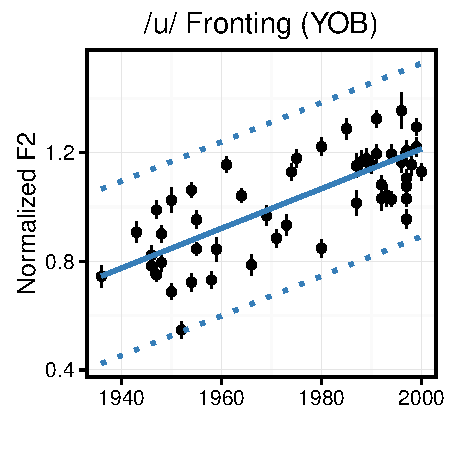
\includegraphics[scale=1.65]{u_fronting_yob.pdf}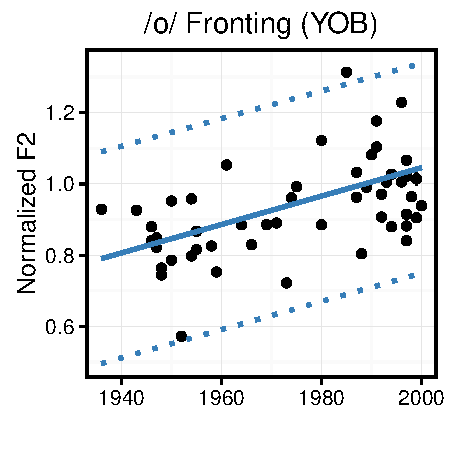
\includegraphics[scale=1.65]{o_fronting_yob.pdf} 
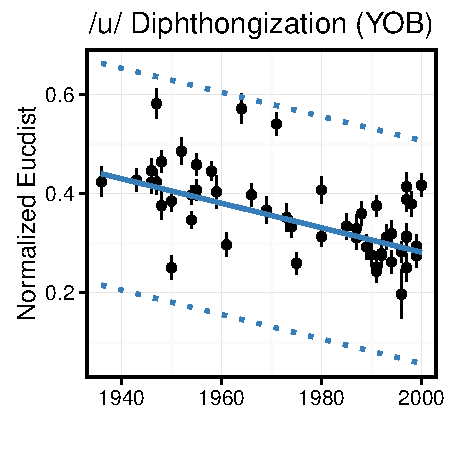
\includegraphics[scale=1.65]{u_dip_yob.pdf}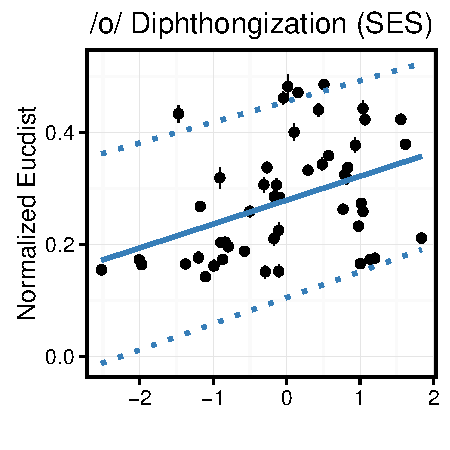
\includegraphics[scale=1.65]{o_dip_soc.pdf}
\end{figure}
\columnbreak
\section*{Method}
\begin{itemize}
\item{Identify a set of social meanings relevant to this community through ethnographic interviews and an open-ended speech evaluation task.}
\item{Measure listeners' ability to match these meanings to variation in the target vowels through a perception experiment.}
\end{itemize}

\begin{figure}[H]
\begin{minipage}{0.25\textwidth}

\raggedright\textit{Figure 1: \textipa{/u/} variants tested (too/food)}\\

\centering
\begin{tabular}{llllll}
&&&&&\\
                  &           & \textit{Fronting}          &             &                   &\\
            &  \multicolumn{3}{l}{$\xleftarrow{\hspace*{15cm}}$  }  &                              \\ \vspace*{-0.3cm}
     \multirow{5}{*}{$\rotatebox[origin=c]{90}{$\underleftarrow{\mathsf{Diphthongization}}$}$}        
                      
 &&&&       &\\
        &\LARGE{\textbf{\textipa{Yu}}}&\LARGE{\textbf{\textipa{0u}}}&\LARGE{\textbf{\textipa{Uu}}}&&\\
                   & High-front  & High-central& High-back\\
               & \LARGE{\textbf{\textipa{eu}}}&\LARGE{\textbf{\textipa{9u}}}&\LARGE{\textbf{\textipa{7u}}}&&\\
       & High-front  & High-central& High-back\\
 & (lowered onset)  & (lowered onset)  &(lowered onset) \\
\end{tabular} 

\normalsize
\vspace*{1cm}
\raggedright\textit{Figure 2: \textipa{/o/} variants tested (toast/so)}\\
\vspace*{-0.25cm}
\centering
\begin{tabular}{llllll}
&&&&&\\
                  &           & \textit{Fronting}          &             &                   &\\
                &  \multicolumn{3}{l}{$\xleftarrow{\hspace*{16cm}}$  }   &                              \\ \vspace*{-0.3cm}
\multirow{5}{*}{$\rotatebox[origin=c]{90}{$\underleftarrow{\mathsf{Diphthongization}}$}$}                 &&&& &                \\
               & \LARGE{\textbf{\textipa{\o:}}}&\LARGE{\textbf{\textipa{8:}}}&\LARGE{\textbf{\textipa{o:}}}&&\\
 & Mid-front  & Mid-central   & Mid-back   &         &          \\
        &\LARGE{\textbf{\textipa{eU}}}&\LARGE{\textbf{\textipa{9U}}}&\LARGE{\textbf{\textipa{oU}}}&&\\
                   & Mid-front   & Mid-central  & Mid-back \\
                   &(fronted onset)&(centralized onset)&(diphthong)&&\\
                   &\LARGE{\textbf{\textipa{9y}}}&\LARGE{\textbf{\textipa{90}}}&&&\\
                   &Mid-front  &Mid-central  &&&\\
                   &(fronted offglide)&(centralized offglide)&&&\\
\end{tabular}
\end{minipage}
\begin{minipage}{0.25\textwidth}
\vspace*{1cm}
\normalsize
\raggedright\textit{Figure 3: Visual stimuli}\\
\vspace*{1cm}

\begin{tabular}{lllll}
\multirow{2}{*}{$\rotatebox[origin=t]{90}{$\overbrace{\rule{2cm}{0pt}\mathsf{\textit{Rural}}\rule{2cm}{0pt}}$\hspace*{-5cm}}$} &
\includegraphics[scale=0.7]{M_O_MC_L_1.png} & 
\includegraphics[scale=0.7]{M_Y_MC_L_1.png} 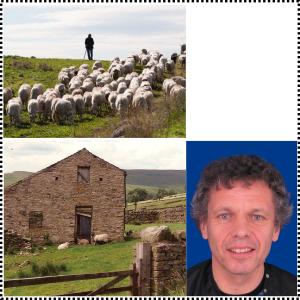
\includegraphics[scale=0.7]{M_O_WC_L_1.png} &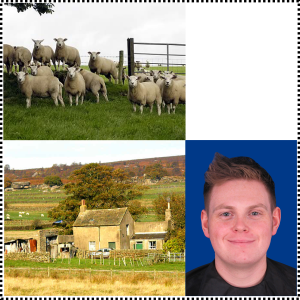
\includegraphics[scale=0.7]{M_Y_WC_L_1.png} \\ \vspace*{-1cm}
 $\rotatebox[origin=t]{90}{\hspace*{3cm}$\overbrace{\rule{2cm}{0pt}\mathsf{\textit{Urban}}\rule{2cm}{0pt}}$}$
    &
\includegraphics[scale=0.7]{M_O_MC_NL_1.png} & 
\includegraphics[scale=0.7]{M_Y_MC_NL_1.png} 
\includegraphics[scale=0.7]{M_O_WC_NL_1.png} & 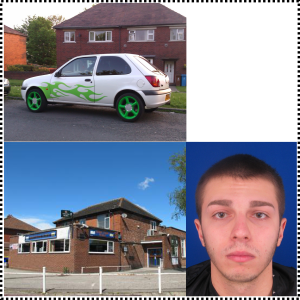
\includegraphics[scale=0.7]{M_Y_WC_NL_1.png}\\\vspace*{-3.5cm}
    &\multicolumn{4}{l}{
$\underbrace{\rule{7cm}{0pt}{\textit{Social class: Middle/Working}}\rule{7cm}{0pt}}$}\\
    &\multicolumn{4}{l}{
    $\underbrace{\rule{3cm}{0pt}{\textit{Age: Older/Younger}}\rule{2cm}{0pt}}$$\underbrace{\rule{3cm}{0pt}{\textit{Age: Older/Younger}}\rule{2cm}{0pt}}$}\\
   
\end{tabular}
\end{sub}
\end{figure}
\vspace{2cm}
\begin{itemize}
\item{\textbf{Task:} \begin{itemize}\item{Participants are told they are listening to an actor pretending to be one of a set of characters in a TV sitcom set in York.}
\item{\textbf{Training phase:} Participants sort the images according to questions e.g. `Which character comes from Rural Yorkshire'?}
\item{\textbf{Testing phase:} Participants see the characters in `minimal pairs', hear a speech token, and select the character which they think the actor is pretending to be.}\end{itemize}}
\item{\textbf{Analysis:}\begin{itemize}\item{Responses analyzed using mixed GLMs with a logit link.}
\item{Models predict the selection of a WC vs MC image as a function of vowel variant heard.}
\item{Individual-level variability modelled through uncorrelated random slopes (variant$|$listener) and random intercepts (listener and item).}\end{itemize}}
\end{itemize}
\normalsize
\columnbreak
\section*{Results}
\subsection*{Main effects for MC/WC selections:}
\centering
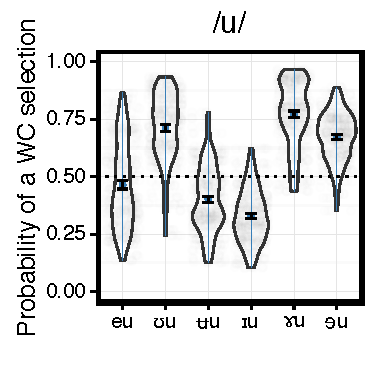
\includegraphics[scale=2.25]{u_fronting_perception_class.pdf}
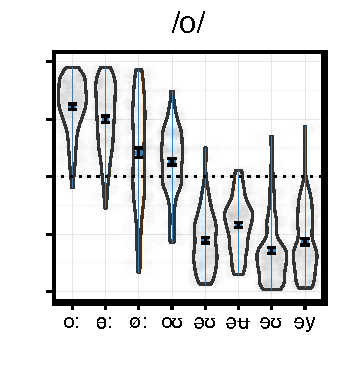
\includegraphics[scale=2.25]{o_fronting_perception_class.pdf}
\begin{itemize}
\item{Listeners perceive back /u/ variants as more `working-class' than fronted variants.}
\item{Additionally, there is a weak effect of /u/ diphthongization, with diphthongal variants heard as more `working-class' than monophthongs.}
\item{Monophthongal /o/ variants cue `working-class' selections.}
\item{Diphthongal /o/ variants cue `middle-class' selections, with the exception of the back dipthongal variant \textipa{[oU]}.}
\item{There is a small effect of fronting within monophthongs -- more fronted variants sound \textit{less} `working-class'.}
\end{itemize}
\justify
\vspace*{-1cm}
\subsection*{How consistent are listeners' intuitions?}
\begin{figure}[H]
\centering
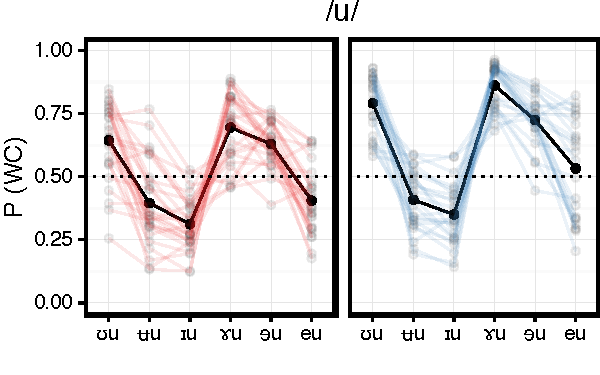
\includegraphics[scale=1.95]{u_clust.pdf}
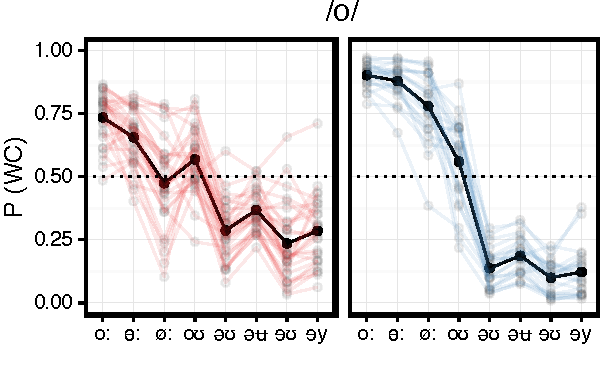
\includegraphics[scale=1.95]{o_clust.pdf}
\end{figure}
\vspace*{-1cm}
%\begin{minipage}{0.4\textwidth}
%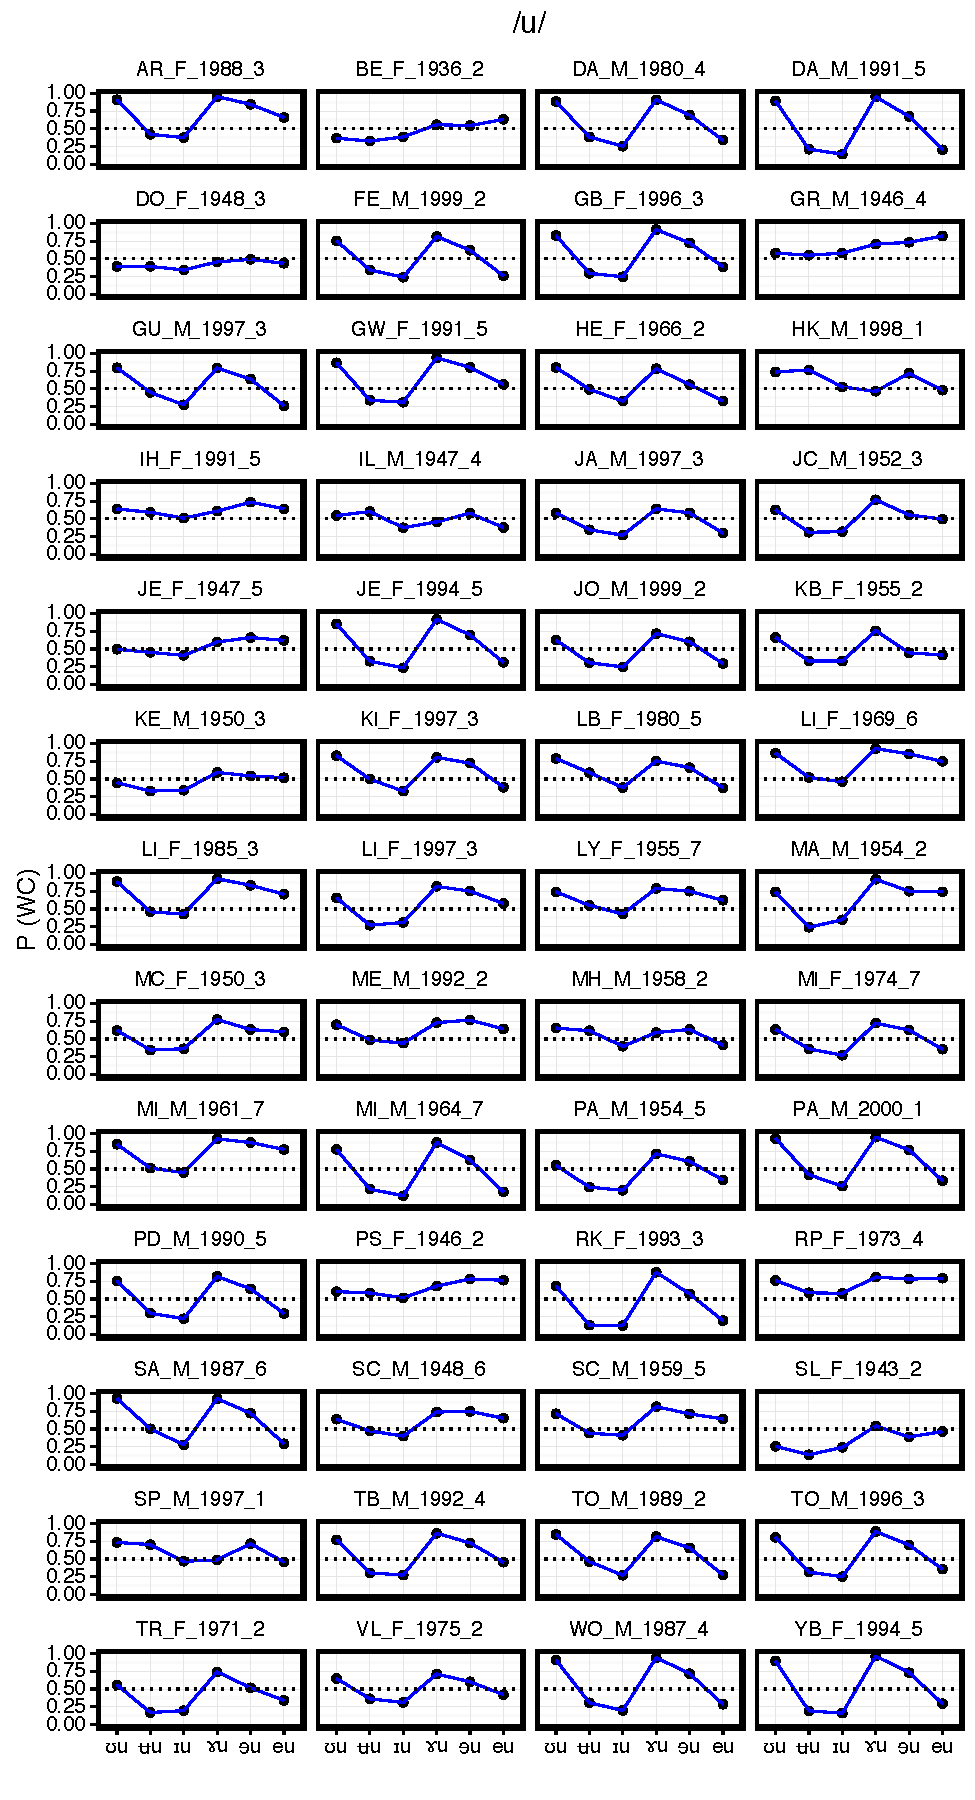
\includegraphics[scale=0.8]{u_ind.pdf}
%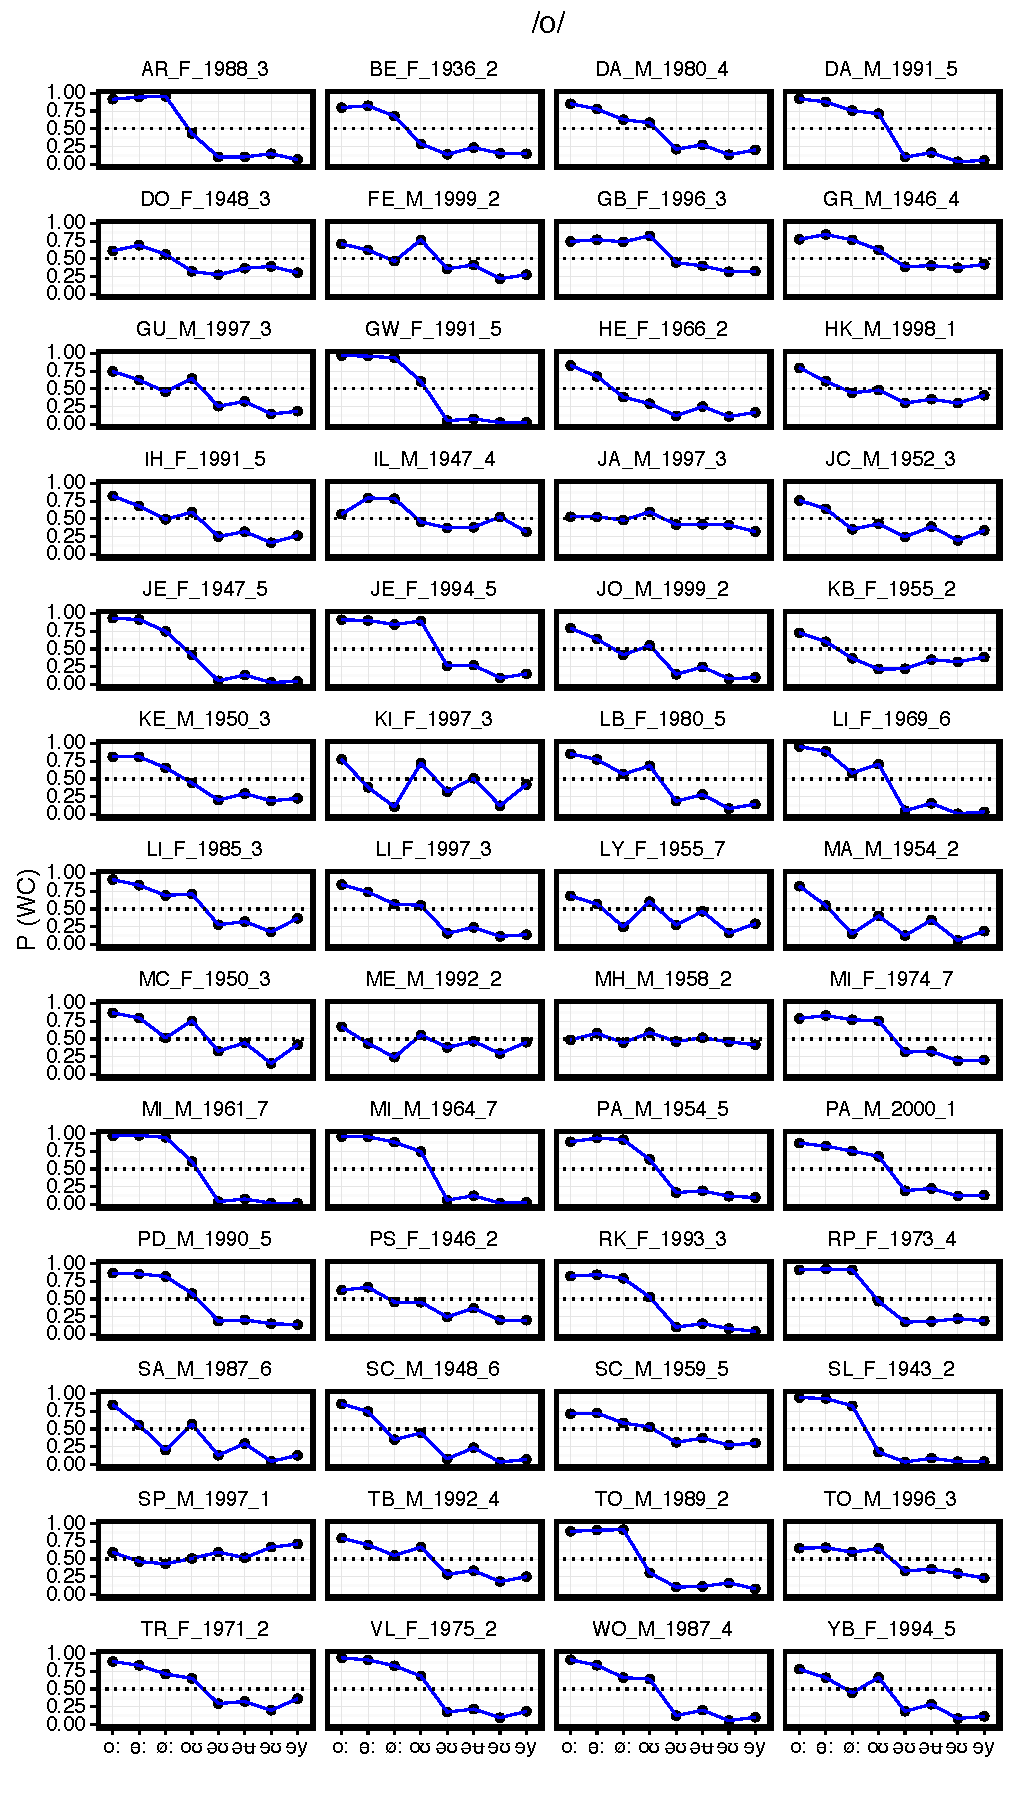
\includegraphics[scale=0.8]{o_ind.pdf}
%\end{minipage}
\begin{itemize}
\item{Responses are similar in directionality, but individuals vary:\begin{itemize}\item{in how much they deviate from chance selections} \item{in terms of which variants they are most sensitive to.}\end{itemize}}
\item{$k$-means clustering reveals at least two perceptual profiles for each vowel:\begin{itemize}\item{For /u/, some listeners are more sensitive to fronting than others (right vs left panel).}\item{/o/ also shows qualitative differences -- some listeners hear \textipa{[\o:]} as relatively unmarked, while others hear it as more `working-class' (left panel vs right panel).}\end{itemize}}
\end{itemize}
\columnbreak
\subsection*{How does this variability relate to social characteristics of the listener?}
\begin{itemize}
\item{Variables tested: Listener gender (M/F); Listener year of birth (1935-2000); Local identity index (-3 +3); Mobility index (-3 +3)}
\end{itemize}
\vspace*{-1cm}
\subsubsection*{/u/: Younger, more mobile listeners are more sensitive to fronting as an index of social class than older, less mobile listeners.}
\hspace*{-1.5cm}
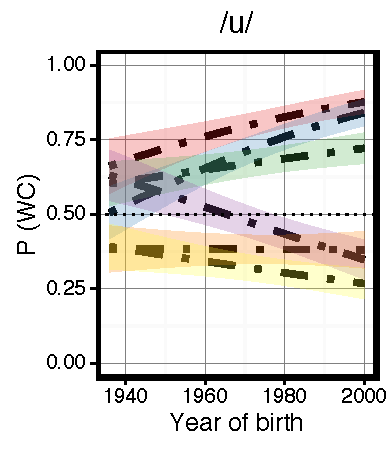
\includegraphics[scale=2]{u_perception_age_sd.pdf}
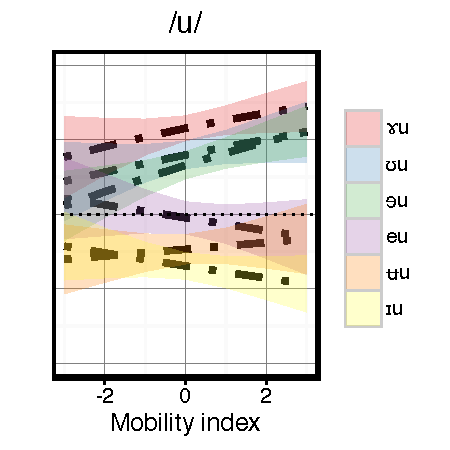
\includegraphics[scale=2]{u_perception_dim3_sd.pdf}
\vspace*{-1.5cm}
\subsubsection*{/o/: More mobile listeners are more sensitive to diphthongization as an index of social class than less mobile listeners.}
\centering
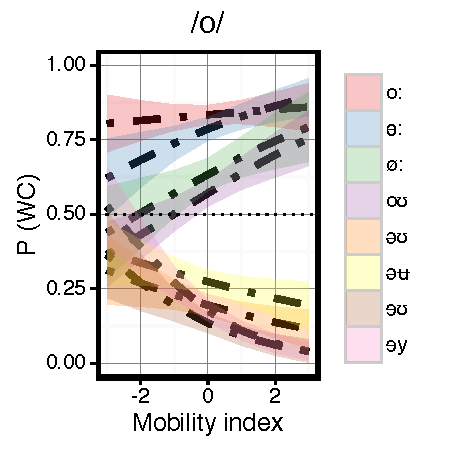
\includegraphics[scale=2]{o_perception_dim3_sd.pdf}
\justify
\vspace*{-2.75cm}
\section*{Conclusion}
\vspace*{-.5cm}
\begin{enumerate}
\item{When interpreting phonetic variation socially, individuals vary:\vspace*{0.5cm}\begin{itemize}\item{...quite a lot in terms of the strength/consistency of their evaluations}\item{...a little in terms of which acoustic dimensions they attend to}\item{...very little in the directionality of their evaluations.}\end{itemize}}
\vspace*{0.5cm}
\item{This variability is related to characteristics of the listener :\vspace*{0.5cm}\begin{itemize}\item{Younger, more mobile listeners are more sensitive to /u/ variation as an index of social class than older, less mobile listeners.}\item{Controlling for age, more mobile listeners are more sensitive to /o/ diphthongization as an index of social class than less mobile listeners.}\end{itemize}}
\end{enumerate}

\vspace*{-1.25cm}
\subsubsection*{References}
\vspace*{-.5cm}
\scriptsize
\begin{description}
\setlength\itemsep{-.25em}
\item[Campbell-Kibler, K. (2008).]{I'll be the judge of that: Diversity in social perceptions of (ING). \textit{Language in Society}, 37(05), 637-659.}

\item[Campbell-Kibler, K. (2009).]{The nature of sociolinguistic perception. Language Variation and Change, 21(01), 135-156.}

\item[Eckert, P. (2008).]{Variation and the indexical field. \textit{Journal of sociolinguistics}, 12(4), 453-476.}

\item[Fridland, V., Bartlett, K., \& Kreuz, R. (2004).]{Do you hear what I hear? Experimental measurement of the perceptual salience of acoustically manipulated vowel variants by Southern speakers in Memphis, TN. \textit{Language Variation and Change}, 16(01), 1-16.}

\item[Grosvald, M. (2009).]{Interspeaker variation in the extent and perception of long-distance vowel-to-vowel coarticulation. \textit{Journal of Phonetics}, 37(2), 173-188.}

\item[Haddican, B., Foulkes, P., Hughes, V., \& Richards, H. (2013).]{Interaction of social and linguistic constraints on two vowel changes in northern England. \textit{Language Variation and Change}, 25(03), 371-403.}

\item[Levon, E., \& Fox, S. (2014).]{ Social Salience and the Sociolinguistic Monitor A Case Study of ING and TH-fronting in Britain. \textit{Journal of English Linguistics}, 42(3), 185-217.}

\item[Munson, B. (2007).]{The acoustic correlates of perceived masculinity, perceived femininity, and perceived sexual orientation. \textit{Language and Speech}, 50(1), 125-142.}

\item[Purnell, T., Idsardi, W., \& Baugh, J. (1999).]{ Perceptual and phonetic experiments on American English dialect identification. \textit{Journal of Language and Social Psychology}, 18(1), 10-30.}


\end{description}
%\bibliographystyle{plain}
%\bibliography{halobib}

\end{multicols}
\end{document}
